\chapter{État de l'art}
Ce chapitre passe en revue les solutions existantes qui parlent d'application des méthodes d'apprentissage pour l'amélioration de la précision de la localisation intérieure. L'exploration de ces sujets va permettre de choisir la solution la plus adaptée pour remplir les objectifs de ce travail.

Pour ce faire, quatre ouvrages ont été étudiés. Les trois premiers traitent du positionnement intérieur aidé avec des algorithmes d'apprentissage (Machine Learning). Le quatrième a été sélectionné, car il traite de la gestion de "outliers", c'est à dire comment détecter des points aberrants et qui pourraient fausser les mesures. 

Grâce à l'étude des structures existantes, une première classification selon le type d'apprentissage et selon les algorithmes de classification utilisés peut être établie. En plus, un aperçu de la façon de détecter les "outliers" est soulevé.

\section{Classification des algorithmes d'apprentissage}
Il existe plusieurs catégories d'estimateur et dans ces catégories, il y a plusieurs algorithmes à choix. La Figure \ref{fig:scikiLearn} permet de sélectionner différents algorithmes en fonction de ce qu'il est nécessaire d'obtenir. On remarque sur cette figure qu'il y a quatre groupes distincts : classification, regression, clustering et dimensionality reduction. En partant depuis le point "start" et en répondant aux différentes questions, cela va proposer un algorithme qui permet de répondre à nos besoins.

\begin{figure}[htp]
 \begin{center}
  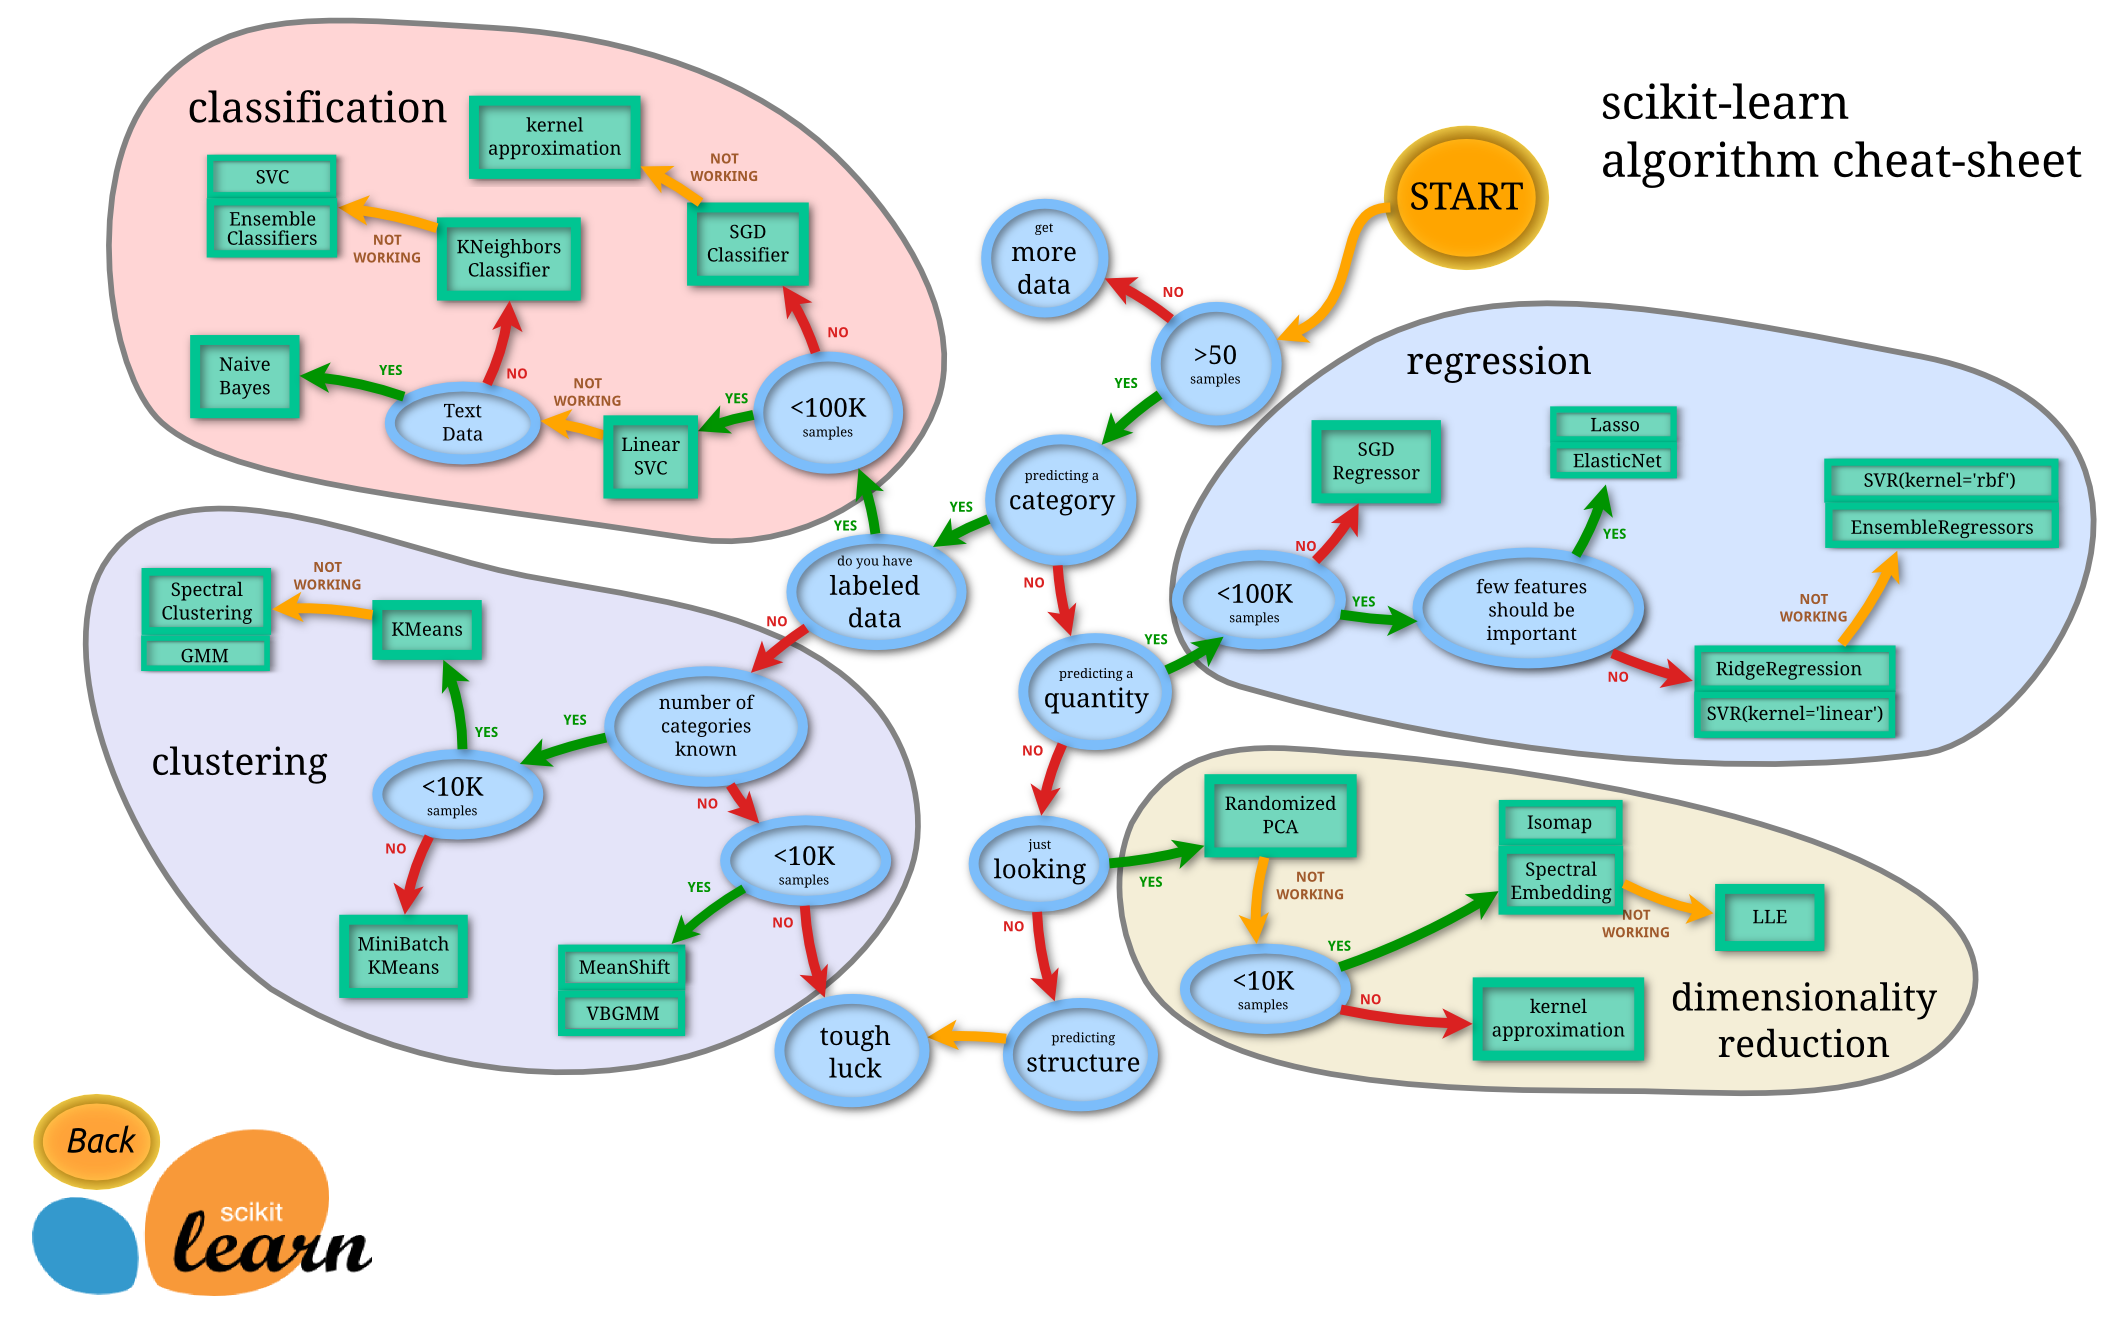
\includegraphics[scale=0.12]{figures/scikiLearn.png}
  \caption{Comment choisir un algorithme ML \cite{scikit}}
  \label{fig:scikiLearn} %% NOTE: always label *after* caption!
 \end{center}
\end{figure}

Dans le cas de ce travail, il y a deux possibilités, soit d'utiliser une classification soit d'utiliser une régression. Dans la Figure \ref{fig:ClassReg}, une petite explication de la différence des deux types d'estimateurs. Dans le cas de la classification, on va apprendre à notre algorithme différentes positions et l'algorithme sera ensuite capable de fournir en sortie une de ses positions. Donc, il sort une région plutôt qu'une coordonnée. Si l'entrainement de l'algorithme a été fait avec un maillage fin alors le résultat sera fin. Lorsqu'un point est détecté, il sera classifié selon la position la plus proche comme on le voit sur la Figure \ref{fig:ClassReg} avec le carré vert et le carré rouge. Dans une régression, la problématique est un peu différente. L'algorithme sera également entrainé avec différentes positions, mais ensuite, par régression l'algorithme va tenter d'estimer la position du nouveau point en calculant sa coordonnée alors que pour une classification il s’agit de positionner ce nouveau point dans une classe. 

\begin{figure}[htp]
 \begin{center}
  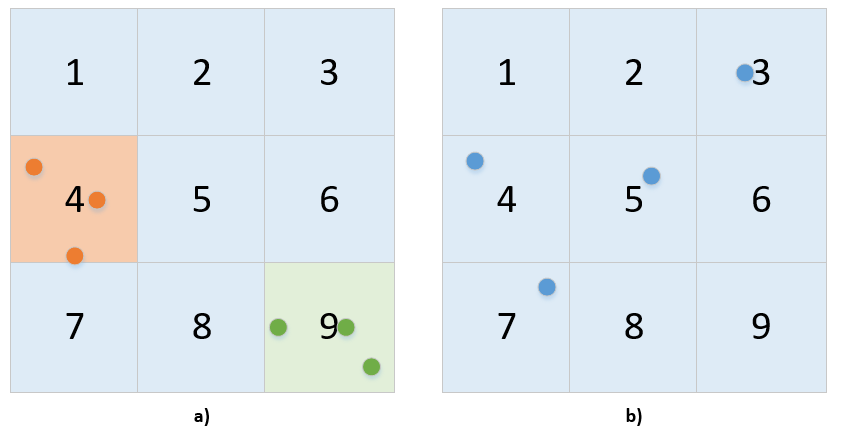
\includegraphics[scale=0.5]{figures/ClassReg.png}
  \caption{a) exemple de classification  b) exemple de régression}
  \label{fig:ClassReg} %% NOTE: always label *after* caption!
 \end{center}
\end{figure}

\section{Algorithme de classification}
Dans cette section, quelques algorithmes de classification utilisés dans ces études \cite{ML_indoor} \cite{CP_RSS} sont brièvement décrits et analysés.

\subsection{Decision Tree}
L'arbre de décisions et une méthode très connue en "machine learning". Il possède des noeuds de décisions (non-terminal), des branches, et des noeuds feuilles (terminal) qui représentent les caractéristiques, condition et les classes. À chaque noeud de décision on sait quelles branches suivre et lorsque l'algorithme atteint un noeud final, le label contenu dans ce même noeud est retourné comme étant la classe. 
L’ID3 de Quinlan et son successeur, C4.5, sont les plus populaires parmi les algorithmes d’arbre de décision \cite{C4_5}.

\subsection{Naïve Bayes}
Le classificateur Naïve Bayes \cite{Bayesian} basé sur le théorème de Bayes est un algorithme d'apprentissage supervisé \cite{DefectPred}. Il est robuste aux données bruyantes, faciles à construire, affiche une grande précision et rapidité lorsqu'il est appliqué à de grandes bases de données et exécute des modèles de classification plus complexes. Par conséquent, il est largement utilisé dans les tâches de classification. Il calcule la probabilité de chaque attribut dans les données en supposant qu'elles sont également importantes et indépendantes les unes des autres. Cette hypothèse est appelée indépendance conditionnelle de classe \cite{KMean_DT} \cite{QUAIL}.

\subsection{Bayesian Network}
L'algorithme de réseau bayésien est largement utilisé pour la classification et est basé sur le théorème de Bayes où la probabilité conditionnelle sur chaque nœud est calculée et forme un réseau bayésien. Il s'appelle également réseau de croyance ou réseau occasionnel. Le réseau bayésien à deux parties nommées qualitatives et quantitatives, qui sont la structure topologique du réseau bayésien et respectivement le tableau de probabilité conditionnelle (CPT) \cite{Bayesian01}.

Le réseau bayésien est un graphe acyclique dirigé où chaque nœud représente un attribut des données et un ensemble de distributions de probabilité. Ces distributions donnent les probabilités pour la valeur de chaque nœud.

\subsection{K-Nearest Neighbor}
Le classificateur K-Nearest Neighbor (K-NN) \cite{ML00} est également connu sous le nom de classificateur basé sur la distance qui classe les instances en fonction de leur similarité. C'est l'un des algorithmes les plus populaires de l'apprentissage automatique. C'est un type d'apprentissage paresseux dans lequel la fonction n'est approchée que localement et tout calcul est retardé jusqu'à la classification. Le point inconnu dans K-NN est assigné à la classe la plus commune parmi ses K-plus proches voisins. Lorsque K = 1, le point inconnu se voit attribuer la classe du point d'apprentissage le plus proche dans l'espace des motifs \cite{ML01}.

\subsection{SMO / SVM}
L'algorithme d'optimisation séquentielle minimale (SMO - Sequential minimal optimization) \cite{ML29} est représenté par John C. Platt pour la formation du classificateur de vecteurs de support à l'aide des noyaux polynomiaux ou RBF. C'est l'un des algorithmes les plus courants pour la classification des grandes marges par SVM. Il remplace globalement toutes les valeurs manquantes et transforme les attributs nominaux en attributs binaires. SVM est une technique de classification basée sur la technologie des réseaux de neuronnes utilisant la théorie de l'apprentissage statistique \cite{ML30}. Il recherche un hyperplan optimal linéaire afin de maximiser la marge de séparation entre la classe positive et la classe négative. En pratique, la plupart des données ne sont pas linéairement séparables; ainsi, pour rendre la séparation possible, la transformation est effectuée à l'aide d'une fonction du noyau. L'entrée est transformée en un espace caractéristique de dimensions supérieures à l'aide d'une cartographie non linéaire. Une décision sur la fonction du Kernel est nécessaire pour implémenter SVM. Le Kernel définit la classe de fonction \cite{ML31}.

\subsection{AdaBoost}
AdaBoost (Adaptive Boosting) \cite{ML32} est un algorithme d'apprentissage d'ensemble. Généralement, il peut être utilisé avec des algorithmes de Machine learning faibles pour améliorer leurs performances. Il est simple à mettre en œuvre, rapide et moins susceptible d'avoir un overfitting. Il améliore les algorithmes de classification instables tels que J48, DecisionStump, etc. L'idée derrière cet algorithme est d'obtenir un classificateur très précis en combinant de nombreux classificateurs faibles. Il fonctionne en exécutant de manière répétée un algorithme d'apprentissage faible donné sur diverses distributions sur les données d'apprentissage, puis en combinant les classificateurs produits par l'apprenant faible en un classificateur composite unique \cite{ML33}. Les classificateurs de l'ensemble sont ajoutés un par un, de sorte que chaque classificateur suivant est entrainé sur des données difficiles pour les membres précédents de l'ensemble. Les poids sont définis sur les instances du jeu de données, en suivant une règle selon laquelle les instances difficiles à classer prennent plus de poids. Cette règle conduit les classificateurs ultérieurs à se concentrer sur eux \cite{ML34}.

\subsection{Bagging}
Le Bagging \cite{ML35} crée des sacs de données de la même taille que le jeu de données d'origine en appliquant une sélection aléatoire à différents sous-ensembles des données d'apprentissage avec de nombreux exemples qui apparaissent plusieurs fois. Ce processus est appelé réplication bootstrap des données d'entrainement. L'idée derrière cette technique est de construire différents classificateurs en utilisant ces sous-ensembles. Chaque sous-ensemble est utilisé pour entrainer un classificateur individuel. Cette approche d'ensemble utilise le nombre de classificateurs a priori \cite{ML35}.

\section{Algorithme de régression}
Dans cette section, quelques algorithmes de régression utilisés dans cette étude \cite{ML_UWB} sont brièvement décrits et analysés.

\subsection{Support Vector Machine pour la régression (SVR)}
Support Vector Machine (SVM) est une méthode d'apprentissage supervisée utilisée pour la classification. Cette méthode peut être étendue pour résoudre des problèmes de régression et cette méthode s'appelle Support Vetor Regression (SVR).

Systeme Vector Regression (SVR) est considéré comme une technique non paramétrique, car il dépend du Kernel. 

Il existe trois implémentations différentes de Support Vector Regression: SVR, NuSVR et LinearSVR. LinearSVR fournit une implémentation plus rapide que SVR, mais ne considère que les noyaux linéaires, tandis que NuSVR implémente une formulation légèrement différente de SVR et de LinearSVR.\cite{scikit}

\subsection{Gaussian Process (GP)}
Gaussian processes a récemment gagné en intérêt du côté des algorithmes d'apprentissage. Cela, car il forme un bon framework pour résoudre des problèmes de régression \cite{ML51}.

C'est une méthode d'apprentissage supervisée pour résoudre des problèmes de régression comme dit ci-dessus, mais également des problèmes de probabilités. 

Les avantages du processus gaussien sont:

\begin{enumerate}
 \item La prédiction interpole les observations (au moins pour les noyaux normaux).
 \item La prédiction est probabiliste (gaussienne) afin que l’on puisse calculer des intervalles de confiance empiriques et décider en fonction de ceux-ci s’il convient de réajuster (adaptation en ligne, adaptation adaptative) la prévision dans une région d’intérêt.
 \item Polyvalent: différents noyaux peuvent être spécifiés. Les noyaux communs sont fournis, mais il est également possible de spécifier des noyaux personnalisés.
\end{enumerate}

Les inconvénients des processus gaussiens sont:

\begin{enumerate}
 \item Ils ne sont pas clairsemés, c’est-à-dire qu’ils utilisent l’ensemble des informations sur les échantillons / caractéristiques pour effectuer la prédiction.
 \item Ils perdent leur efficacité dans les espaces de grandes dimensions, notamment lorsque le nombre de caractéristiques dépasse quelques dizaines.
\end{enumerate} 

\cite{scikit}. 

\section{ Détection d'outliers \cite{ML_indoor}}
Cette section donne un aperçu de la manière de traiter les "outliers - valeurs aberrantes", c'est-à-dire les points qui ne sont pas cohérents lors d'une mesure. Selon Barnet et Lewis \cite{Outliers}, un "outliers" est défini comme étant une observation qui semble incompatible avec le reste d'un ensemble de données.
Garder un "outliers" dans un jeu de données peut amener à de mauvais résultats, il est donc important de les détecter correctement. Il existe différentes méthodes pour déterminer ces "outliers" :

\begin{enumerate}
 \item Grubbs' test : détecte un "outliers" en supposant une distribution normale.
 \item Tietjen-Moore test : C'est une généralisation de Grubbs' test pour détecter de multiple outliers. Il a cependant un inconvénient, il est nécessaire de connaitre le nombre exact d'ouliers.
 \item Generalized Extreme Studentized Deviate (ESD): c'est également une généralisation du test Grubbs', mais il n'est pas nécessaire de connaitre à l'avance le nombre d'ouliers. Ce test nécessite uniquement une limite supérieure pour le nombre suspect d'outliers.\cite{ESD}
\end{enumerate}

\section{Étude des travaux existants}
Les trois documents ne peuvent pas être comparés à proprement dit, car ils traitent de différentes manières. Un parle d'algorithme de classification et compare différents algorithmes existants. Un autre document traite de régression et compare également différents algorithmes. Le dernier document parle de la prédiction conforme (CP - conformal prediction) qui va permettre d'améliorer encore les résultats avec un algorithme choisi.  

C'est pourquoi les documents sont résumés en mettant les points importants en évidence séparément. Ils seront décrits plutôt que comparés. 

\subsection{Analyse comparative de différents algorithmes pour le positionnement intérieur \cite{ML_algo}}
Cette publication parle d'une analyse comparative entre différents algorithmes de "machine learning" pour du positionnement intérieur. L'étude est basée sur un positionnement "fingerprint" ce qui permet de cartographier un endroit à l'aide de la force du signal réceptionné (RSS - Received Signal Strength).
Dans cet article, les algorithmes de "machine learning" sélectionnés sont comparés en termes de précision de positionnement et de temps de calcul. 

Au cours des expériences, la base de données UJIIndoorLoc est utilisée. La classification est effectuée en premier lieu en utilisant le jeu de données d'origine en considérant les valeurs RSS des 520 points d'accès sans fil (WAP - wireless access points) et les nouveaux attributs définis en tant que «cellule» qui composent les attributs : BuildingID, Floor, SpaceID et RelativePos. Ensuite, une nouvelle méthode est proposée: «Séparation déductive pour le positionnement intérieur (DESIP - Deductive Separation for Indoor Positioning)». Dans cette méthode, tout d'abord, seules les informations de bâtiment et les valeurs RSS mesurées à partir de 520 WAP sont utilisées pour la tâche de classification.

Durant les expériences, des algorithmes tels que le plus proche voisin (NN - nearest neighbor), le SMO, l'arbre de décision (J48), Naïve Bayes et Bayes Net sont utilisés. L’algorithme le plus approprié pour la solution du problème de positionnement intérieur est déterminé en comparant la précision et le temps de calcul de chaque approche.

La base de données entière est séparée de telle sorte que 19'937 enregistrements soient réservés à l'apprentissage et 1'111 enregistrements soient réservés aux tests. Il y a 529 caractéristiques qui sont: les coordonnées où sont prises les empreintes digitales WiFi, telles que bâtiment, étage, espace (bureau, laboratoire, etc.), position relative (dans une pièce ou dans un couloir), etc. Le jeu de données d'apprentissage UJIIndoorLoc comprenant les valeurs RSSI de 520 WAP et une autre «cellule» qui comprend les attributs floor, buildingID, spaceID et relative position de l'ensemble de données d'origine est utilisé pour la tâche de classification. Les étapes des expériences utilisant ce jeu de données sont illustrées à la Figure \ref{fig:newAttribute}. Dans un premier temps, le jeu de données (dataset) est séparé en deux groupes. Un groupe est utilisé pour l'apprentissage (train dataset) et l'autre partie est utilisée pour valider le résultat des différents algorithmes (test dataset). Le jeu d'entrainement est utilisé pour quatre différents algorithmes.

\begin{figure}[htp]
 \begin{center}
  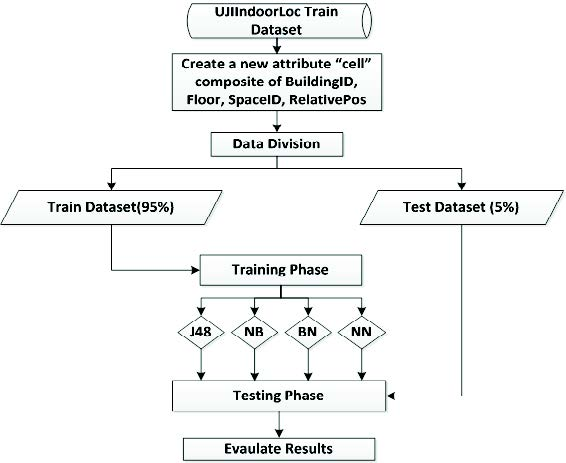
\includegraphics[scale=0.7]{figures/newattribute.jpg}
  \caption{Phase de construction et d'apprentissage \cite{ML_algo}}
  \label{fig:newAttribute} %% NOTE: always label *after* caption!
 \end{center}
\end{figure}

Dans cet article, les algorithmes suivants ont été comparés dans différentes situations: NN, SMO, J48, Naïve Bayes et BayesNet. La classification est effectuée en trois phases (building,floor and region). La première étape est la classification par bâtiment (Figure \ref{fig:builClass}). Le résultat des algorithmes pour cette classification donne BayesNet comme étant le meilleur, car il possède la meilleure précision.

\begin{figure}[htp]
 \begin{center}
  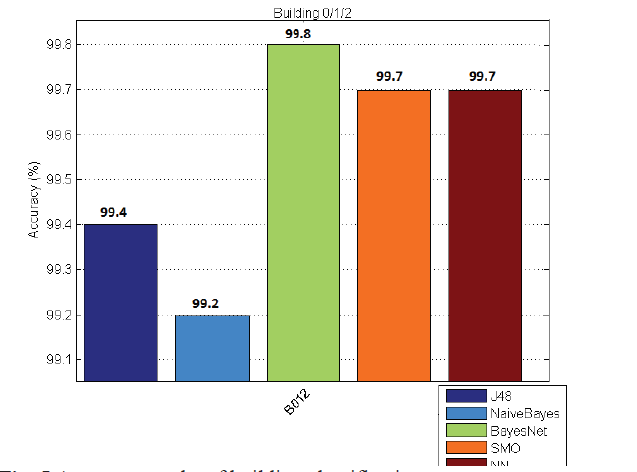
\includegraphics[scale=0.6]{figures/bluildingClassification.png}
  \caption{Résultats des précisons pour la classification par bâtiments \cite{ML_algo}}
  \label{fig:builClass} %% NOTE: always label *after* caption!
 \end{center}
\end{figure}

Suite à cela, la classification a été faite en fonction des étages (floors) (Figure \ref{fig:floorClass}). Dans ce cas, le meilleur algorithme est NN. 

\begin{figure}[htp]
 \begin{center}
  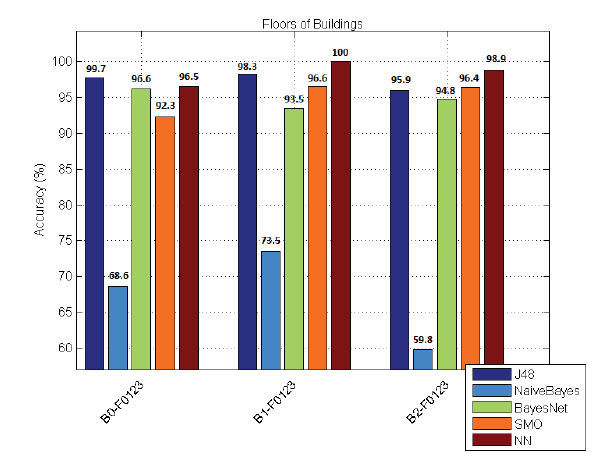
\includegraphics[scale=0.6]{figures/floorClassification.png}
  \caption{Résultats de la précision pour la classification par étage.\cite{ML_algo}}
  \label{fig:floorClass} %% NOTE: always label *after* caption!
 \end{center}
\end{figure}

Et pour la dernière étape (Figure \ref{fig:regionClass}), la classification a été faite en fonction de la région et là encore, c'est l'algorithme NN qui est le meilleur.

\begin{figure}[htp]
 \begin{center}
  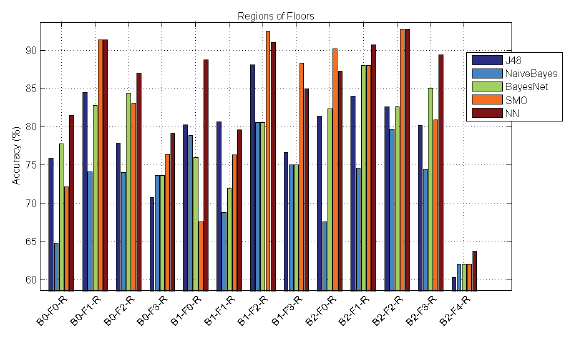
\includegraphics[scale=0.6]{figures/regionClassification.png}
  \caption{Résultats de la précision pour la classification par région. \cite{ML_algo}}
  \label{fig:regionClass} %% NOTE: always label *after* caption!
 \end{center}
\end{figure}

Les deux tableaux (Figure \ref{fig:accuracy} et Figure \ref{fig:time}) permettent d'avoir une vue d'ensemble de tous les algorithmes appliqués et leur performance en termes de précision et de rapidité. L'algorithme NN est le meilleur pour tous les jeux de données au niveau du temps d'exécution. En ce qui concerne la précision, Bayes Net est meilleur pour la classification "building" par contre NN est meilleur dans tous les autres cas.

\begin{figure}[htp]
 \begin{center}
  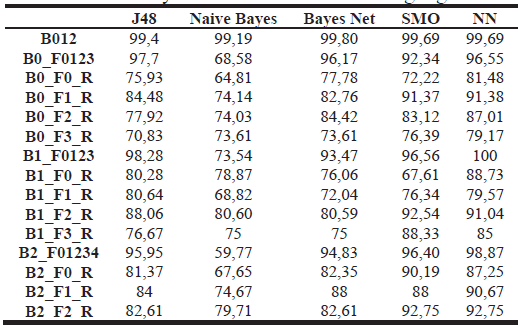
\includegraphics[scale=1]{figures/accuracy.png}
  \caption{Résultat de la précision des algorithmes d'apprentissage.\cite{ML_algo}}
  \label{fig:accuracy} %% NOTE: always label *after* caption!
 \end{center}
\end{figure}

\begin{figure}[htp]
 \begin{center}
  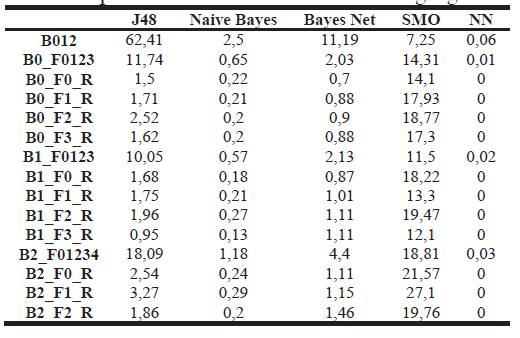
\includegraphics[scale=1]{figures/time.png}
  \caption{Résultats du temps de traitement des algorithmes d'apprentissage\cite{ML_algo}}
  \label{fig:time} %% NOTE: always label *after* caption!
 \end{center}
\end{figure}

Les résultats expérimentaux révèlent que l’algorithme k-Nearest Neighbor (k-NN) est le plus approprié lors du positionnement. En outre, J48 offre des performances quasiment identiques lorsqu'il est utilisé avec des algorithmes itératifs, à savoir AdaBoost et Bagging. Il est à noter que toutes ces méthodes mettent en évidence des classifications. C'est-à-dire que le résultat placera un nouveau point sur l'un des points entrainé et ne donne pas une nouvelle coordonnée comme cela serait le cas d'un résultat par régression. 

\subsection{Machine learning pour diminuer l'erreur de positionnement UWB \cite{ML_UWB}}
Les approches classiques pour faire face au défi de localisation dans des environnements encombrés impliquent généralement d'abord la détection de la condition NLOS (NLOS = pas en ligne de vue), puis la prise de mesures appropriées pour prendre en compte la condition NLOS. Toutefois, la grande variété de matériaux et d’environnements d’exploitation variés peuvent impacter les performances de la mesure de ranging, ce qui indique que la distinction entre LOS et NLOS n’est pas toujours significative. Sur la base de cette observation, ils ont opté pour une approche différente dans cet article. Leur approche utilise des techniques de Machine Learning non paramétriques (SVM et GP) pour estimer l’erreur de "ranging" directement à partir de la forme d’onde reçue, sans aucune connaissance a priori ou a posteriori de la condition NLOS. 

Cette publication traite de la diminution de l'erreur du mode ranging concernant la localisation UWB (Ultra Wide Band). Plusieurs techniques existent pour diminuer l'erreur de positionnement en détectant ce qui est en ligne de vue (LOS) ou non (NLOS). Ici, une autre technique est exploitée et va directement diminuer cette erreur que ça soit en LOS ou en NLOS. Ils appliquent deux classes de régresseurs non paramétriques pour avoir une estimation de l'erreur de mesure. Afin de valider leurs résultats, ils ont fait une vaste campagne de mesures intérieures. Cette technique montre une amélioration de performances significatives dans divers scénarios par rapport aux approches conventionnelles. 

La régression non paramétrique est une forme d'analyse de la régression dans laquelle le prédicteur, ou fonction d'estimation ne prend pas de forme prédéterminée, mais est construite selon les informations provenant des données. La régression non paramétrique exige des tailles d'échantillons plus importantes que celles de la régression basée sur des modèles paramétriques parce que les données doivent fournir la structure du modèle ainsi que les estimations du modèle. \cite{WIKI1}

Ils se sont appuyés sur des outils d'apprentissage (Machine Learning), et proposent deux techniques de régression pour estimer l’erreur de mesure, en se basant uniquement sur la forme d’onde reçue et la distance estimée.

\begin{enumerate}
 \item La première technique utilise une régression SVM (support vector machine) pour trouver un hyperplan qui se rapproche de l'erreur de mesure en fonction des données d'apprentissage. 
 \item La seconde technique utilise un processus gaussien (GP) pour déterminer la distribution a posteriori de l'erreur de mesure, en fonction des données d'apprentissage. 
\end{enumerate}

L'erreur de mesure estimée, associée à une mesure de certitude, peut être transmise à un algorithme de localisation. Leurs techniques de régression présentent l'avantage supplémentaire de pouvoir être appliquées même lorsque les données d'apprentissage ne sont pas étiquetées avec des informations LOS ou NLOS.

Lors des mesures, il existe beaucoup de paramètres qui peuvent créer une erreur. Avec un seul modèle, il est difficile de capturer tous les types de perturbations. Dans cette publication, ils se basent sur 1024 mesures (512 LOS et 512 NLOS) Figure \ref{fig:LosNlos}.

\begin{figure}[htp]
 \begin{center}
  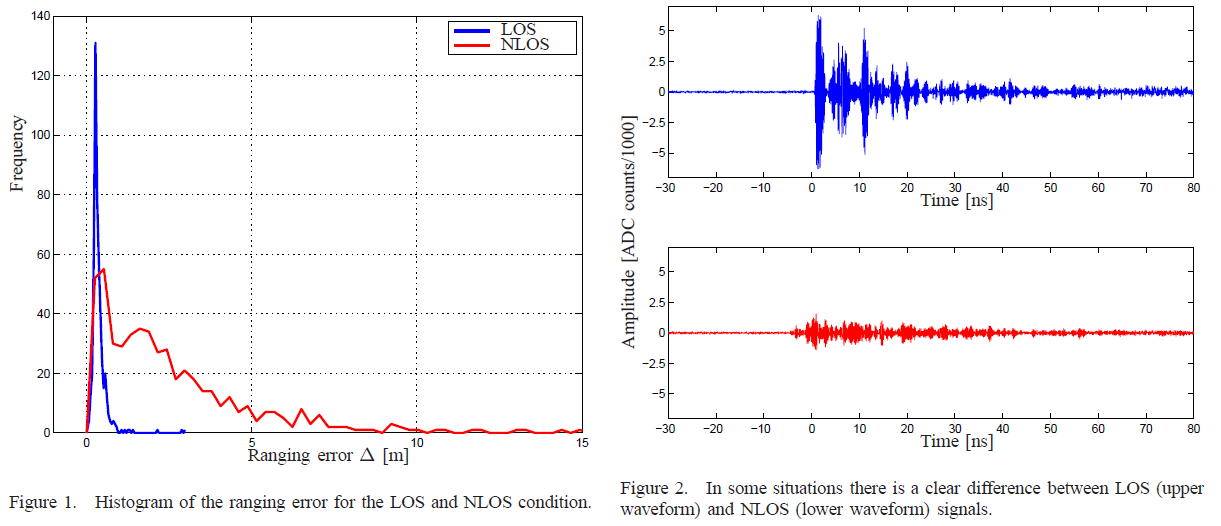
\includegraphics[scale=0.6]{figures/LosNlos.png}
  \caption{Ranging error - LOS and NLOS \cite{ML_UWB}}
  \label{fig:LosNlos} %% NOTE: always label *after* caption!
 \end{center}
\end{figure}

Sur la base d'une vaste campagne de mesures en intérieur avec des radios UWB conformes à la FCC (Federal Communications Commission), ils ont évalué les performances de localisation en termes de probabilité de panne pour différentes stratégies de localisation. Leurs résultats ont révélé que: 

\begin{enumerate}
 \item La minimisation de l1-norme est plus robuste pour faire face aux valeurs aberrantes (outliers) que la minimisation de l2-norme, pour une localisation sans atténuation.
 \item les contraintes peuvent générer des gains significatifs, en particulier lorsque les exigences de localisation ne sont pas trop strictes.
 \item les techniques de régression SVM ou GP offrent des gains de performance supplémentaires pour tous les scénarios considérés.
 \item Les techniques de régression SVM ou GP, combinées à la connaissance des contraintes relatives à l'erreur de "ranging", offrent les meilleures performances pour les scénarios considérés.
\end{enumerate}

\subsection{Amélioration du positionnement en utilisant "conformal prediction" \cite{CP_RSS}}
Pareil que dans les deux précédentes publications, le but est d'améliorer la précision du positionnement intérieur où il n'est pas possible d'utiliser un GPS. Cela toujours en tenant compte des problématiques d'un environnement dynamique avec des personnes qui bougent et de l'environnement complexe avec des murs, etc.. Dans cet article, ils ont validé leur solution dans trois immeubles. Cet article est basé sur un positionnement WIFI fingerprinting et se base sur la force du signal reçu (RSSI).

Pour effectuer les mesures il y a deux phases voir Figure \ref{fig:Fingerprinting}. 

\begin{figure}[htp]
 \begin{center}
  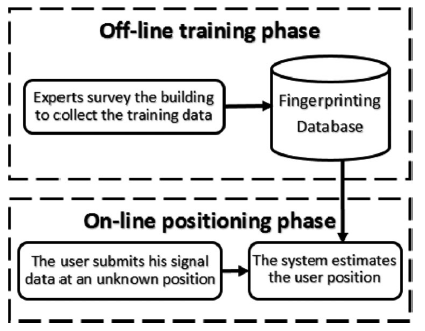
\includegraphics[scale=1]{figures/Fingerprinting.png}
  \caption{Les deux phases du fingerprinting}
  \label{fig:Fingerprinting} %% NOTE: always label *after* caption!
 \end{center}
\end{figure}

La première phase (Off-line training) consiste à décider combien de mesures nous voulons faire (tous les mètres? centimètres?), comment sont prises les mesures (plusieurs mesures sont faites à chaque position) et comment labéliser le signal (souvent labélisé avec la coordonnée réelle). Cette phase est très importante et il est nécessaire de bien réfléchir comment procéder (utiliser un robot par exemple). C'est ce qu'on appelle la phase d'entrainement.

Concernant la seconde phase (on-line positioning), c'est de définir le positionnement. Durant cette phase la partie délicate est de définir quel algorithme utiliser. C'est durant cette phase que les algorithmes seront testés. 

Il existe une compétition comparative pour les positionnements intérieurs (Microsoft IPSN 2014) Figure \ref{fig:Competition}.

Une localisation précise à l'intérieur peut potentiellement transformer la façon dont les gens naviguent à l'intérieur, de la même manière que le GPS a transformé la façon dont les gens naviguent à l'extérieur. Au cours des 15 dernières années, le monde universitaire et l’industrie ont proposé et expérimenté plusieurs technologies de localisation en intérieur, mais nous n’avons pas encore assisté à des déploiements à grande échelle. Ce concours vise à rassembler des technologies de localisation intérieure en temps réel ou quasi réel et à comparer leurs performances dans le même espace. \cite{MICRO}

\begin{figure}[htp]
 \begin{center}
  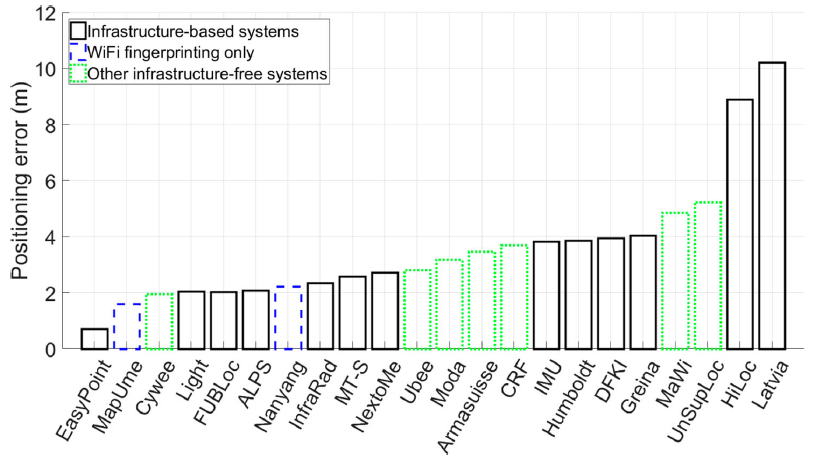
\includegraphics[scale=0.6]{figures/Competition.png}
  \caption{Performance de la précision du fingerprint lors de la compétition Microsoft IPSN 2014 competition \cite{CP_RSS}}
  \label{fig:Competition} %% NOTE: always label *after* caption!
 \end{center}
\end{figure}

Cela permet de mettre en évidence les précisions qui sont obtenues. Les algorithmes qui seront étudiés sont : Weighted K-nearest neighbours (W-KNN), Naïve Bayes Figure \ref{fig:PerfAccu}. Tous les mesures et tests sont basés sur le RSS du WIFI. 

\begin{figure}[htp]
 \begin{center}
  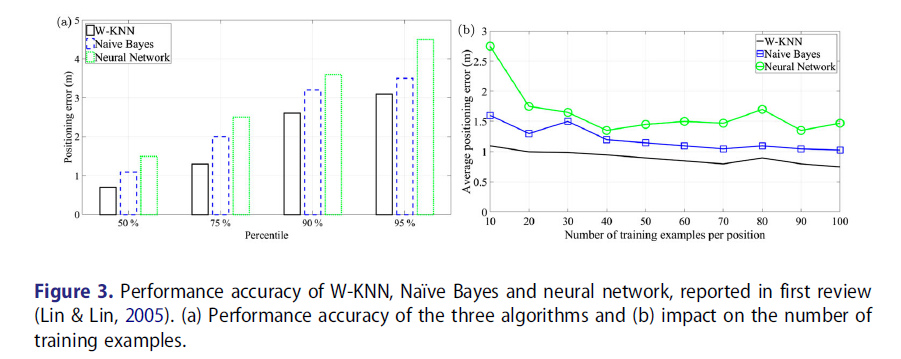
\includegraphics[scale=1]{figures/PerfAccu.png}
  \caption{Performance de la précision de W-KNN, Naïve Bayes et réseau de neurones, mais aussi l'impacte du nombre de données d'entrainement\cite{CP_RSS}}
  \label{fig:PerfAccu} %% NOTE: always label *after* caption!
 \end{center}
\end{figure}

Les mesures ont été effectuées de trois manières différentes (dans un corridor, sur un étage, sur trois étages - voir dans le document  \cite{CP_RSS}). En résumé, la synthèse des trois solutions suggère que, avec uniquement la mesure métrique WiFi RSS, de nombreux algorithmes complexes risquent de ne pas être aussi performants que des algorithmes plus simples. Malgré sa simplicité, W-KNN a excellé dans la plupart des analyses de "fingerprinting". Il convient de noter que le système MapUme, deuxième sur vingt-deux concurrents du concours Microsoft IPSN 2014, utilisait également W-KNN comme principal algorithme. Cependant, l'approche Naïve Bayes améliore sa précision lorsque le nombre d'entrainements est élevé, ce qui indique qu'au-delà du WiFi RSS, des informations supplémentaires seront nécessaires pour améliorer davantage les performances du "fingerprinting".

Une chose qui est également importante c'est la confiance qu'il y a dans un algorithme. Pour cela, cet article a utilisé "conformal prediction (CP)" afin de donner un indice de confiance. Plus la confiance est souhaité, plus il est nécessaire d'avoir de jeu de données. Les avantages d'utiliser l'indice de confiance sont les suivants:

\begin{enumerate}
 \item Chaque prédiction est associée à un indice de confiance et permet de dire combien la prédiction est correcte. 
 \item La prédiction produite par CP est statistiquement correcte sous les paramètres qui ont été choisis dans la phase on-line.
 \item le niveau de confiance peut être ajusté pour produire un ensemble de prédiction plus grand ou plus petit.
\end{enumerate}

Afin de valider leur algorithme, ils ont utilisé trois bancs de test Figure \ref{fig:TestBed}. 

\begin{enumerate}
 \item Royal Holloway : Données récoltées manuellement dans un office standard avec un smartphone
 \item Cambridge : Données récoltées automatiquement par un robot dans un environnement assez idéal.
 \item UJIIndoorLoc : Utilise le dataset public qui couvre une grande surface intérieure basée sur trois bâtiments.
\end{enumerate}

\begin{figure}[htp]
 \begin{center}
  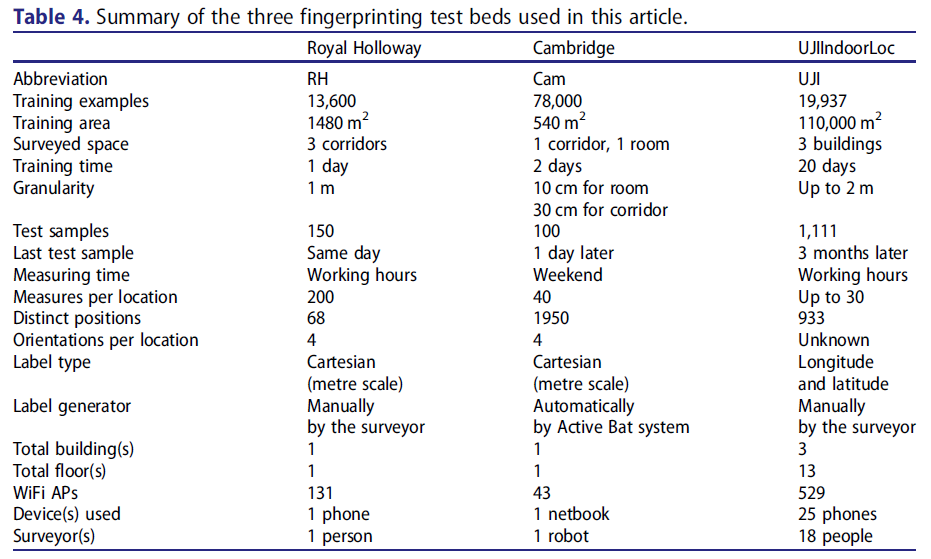
\includegraphics[scale=0.5]{figures/TestBed.png}
  \caption{Summary of the three fingerprinting test beds used in this article \cite{CP_RSS}}
  \label{fig:TestBed} %% NOTE: always label *after* caption!
 \end{center}
\end{figure}

Pour résumer cet article, il propose une nouvelle approche d'apprentissage basé sur la confiance d'un algorithme permettant d'estimer la position de l'utilisateur à l'intérieur avec la force du signal WiFi. Il introduit une mesure de confiance, non seulement utile pour refléter l'incertitude des prédictions de positionnement, mais également capable d'ajuster la taille de l'ensemble de prédictions en conséquence. 

Il a été montré empiriquement que la précision de positionnement était d’environ 2,4 m / probabilité de 75\% avec un banc d’essai normal, environ 70 cm / probabilité de 75\% avec un banc d’essai idéal et d’environ 8,8 m / probabilité de 75\% avec un banc d’essai difficile. 

Ces résultats ont surpassé les algorithmes de Machine Learning sans indice de confiance mis à l'essai sur les mêmes bancs d'essai jusqu'à 20\% plus précis. Si l'on ne tient pas compte de CP, l'algorithme W-KNN est un peu meilleur que Naïve Bayes. 

Les approches présentées dans cet article ne nécessitent pas de carte du bâtiment. Cela pourrait être utile de les avoir afin d'avoir des informations supplémentaires pour supprimer les mauvaises prédictions comme par exemple une personne qui marche dans un mur alors qu'elle est dans le couloir.

\section{Choix et conclusion}
Le choix de l'algorithme suite à l'analyse de l'état de l'art est une tâche difficile. Il est important de garder en tête l'application finale pour laquelle le système sera utilisé, c'est-à-dire, pour faire du positionnement intérieur.

En premier lieu, il est nécessaire de choisir entre un apprentissage par classification ou par régression. Il est clair que pour une utilisation finale un algorithme traitant de la régression comme SVM serait le mieux adapté. Ceci afin d'entrainer le système avec peu de positions et d'estimer les autres positions.

Cependant, il n'est pas vraiment réaliste de démarrer directement avec une technique pareil sans même savoir si les données disponibles sont exploitables. C'est pourquoi la décision a été de démarrer avec un algorithme de classification dans l'optique d'améliorer le système avec un algorithme de régression.

Suite, à l'étude des documents existants, il aurait été possible de sélectionner l'algorithme KNN qui a donnée dans la plupart des cas de bons résultats. Mon choix c'est dirigé vers l'algorithme SVM qui est également bien classé. Ce choix a été fait en grande partie, car il est également cité pour la régression en tant que SVR alors que KNN est uniquement cité pour de la classification. 

%\begin{enumerate}
% \item fgfd
% \item gdgfd
%\end{enumerate}


%\begin{figure}[H]
% \begin{center}
%  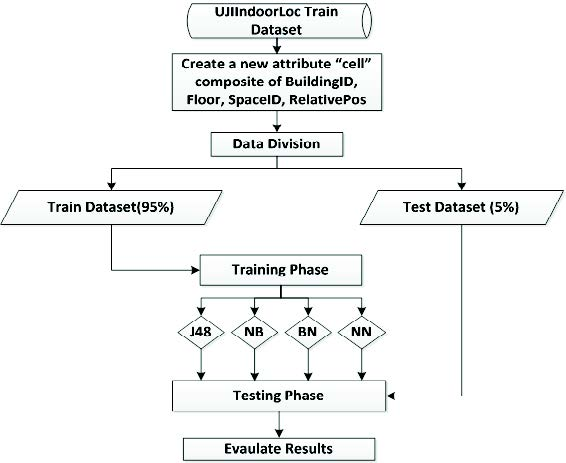
\includegraphics[scale=1]{figures/newattribute.jpg}
%  \caption{The new attribute “cell” construction phase}
%  \label{fig:newAttribute} %% NOTE: always label *after* caption!
% \end{center}
%\end{figure}

%\todo{Compléter cette partie qui semble importante}

